\chapter{Mathematical Background}\label{chapter:math}

Next, to address the practical part of the thesis, it is needed to give some attention to the underlying math. Considering that the system described in chapter \ref{chapter:implementation} extensively uses techniques and concepts from the field of digital signal processing, it was decided to make a brief introduction to the basics of it for a reader that might be confused by the variety of new terms. Thus, the present chapter will firstly describe how sounds are represented computationally, and then will provide a few examples of the most common ones. Next, a section dedicated to digital filters and filterbanks will follow, and finally, some other mathematical concepts used in the implementation part will be addressed.

\section{The Basics of Digital Signal Processing}\label{section:math_basics}

As it was described in chapter \ref{section:physics_sound}, physical sounds in real world spread in the environment in a form of pressure waves. These waves are continuous, thus to be able to work with sounds via computers it is usually useful to convert them to some kind of a discrete representation. The notion of a discrete, or discrete-time, signal is used here and is defined as a time series sampled at equally-spaced points on the time axis, or as a function of discrete time (for example, $x(n)$) \cite{Shenoi2005}. Digital signals are, in simple words, encoded representations of the discrete-time signals. The digital signal's sampling frequency $f_s$ is defined as a number of samples observed during a unit of time. Sometimes, digital signals are represented as vectors \cite{Abood2020}: \begin{equation}
	\textbf{x} = [x(0), x(1), \dots{}, x(N - 1)]^T\qquad\textbf{x}\in\mathbb{R}^N
\end{equation}
where $N$ is overall number of samples.\\

If you recall the conversation about resonant frequencies and the sinusoidal manner of vibrations from chapter \ref{section:physics_sound}, you may remember that when an impulse is delivered to an object, the object responds to it by entering into vibrations. It starts to vibrate at all possible frequencies, but not all of them survive. An important mathematical instrument for frequency analysis is Fourier transform (along with Fourier series). Fourier theorem states that any periodic function might be represented as a sum of sines and cosines, so technically, any waveform of a sound (including the ones for sound waves) might be decomposed and represented in such a way. This decomposition may also be given by an amplitude spectrum and a phase spectrum \cite{Schnupp2011}.\\

The most basic example of such frequency decomposition is for a pure tone (the first row on figure \ref{img:windowing_example}). Pure tones are impossible to find in nature, or even perfectly produce with a speaker. Pure tones produced computationally sound flat and unnatural, but they are the basic building blocks of other sounds. The waveform of a pure tone is a sine wave and is defined as a function of time $t$:
\begin{equation}
	y(t) = a\sin(2\pi{}ft + \varphi)
\end{equation}
where $f$ is the frequency, $a$ is the amplitude and $\varphi$ is the phase. The frequency decomposition of a pure tone will contain only one peak at frequency $f$.\\

Another example of a common sound would be a click. Clicks are instant modulations in amplitude of a sound waveform, or waves that instantly go up and down at certain points in time. The most interesting fact about a click is its frequency decomposition being an infinite set of sine waves. More about clicks can be found, for example, in \cite{Schnupp2011}.\\

The last important sound that will be mentioned here is white noise. The waveform of a white noise is completely random, so its frequency decomposition is random too. White noise is used in the thesis for experiments with the resulting CASA system and its ability to separate music.\\

Continuing the conversation about frequency decomposition, it is necessary to note that it is impossible to extract any information about the time component from the output of the Fourier transform. Thus, it is useful to firstly split the wave into separate intervals on the time axis (which are often called windows), and only then compute their frequency decompositions. The resulting time-frequency representation of the sound wave is called spectrogram. An example of a spectrogram is shown on figure \ref{img:spectrogram_example}.

\begin{figure}[h]
	\centering
	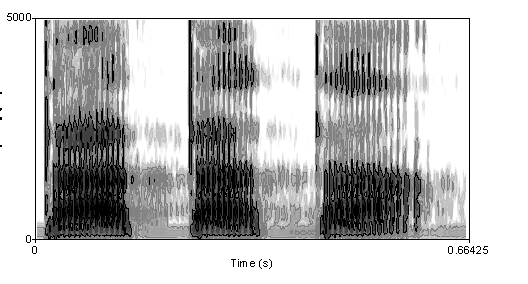
\includegraphics[height=0.25\textheight]{include/spectrogram_example}
	\caption[An example of a spectrogram]{A spectrogram of a male voice saying "ta-ta-ta". Time is shown on the horizontal axis, and frequencies are shown on vertical. The color intensity increases with density. Three separate syllables are clearly visible. Taken from \url{{https://commons.wikimedia.org/}}}
	\label{img:spectrogram_example}
\end{figure}

However, there is a known problem that emerges when windowing is used with the Fourier transform. When the window is rectangular (the wave is cut off vertically from both sides) and is not aligned with the period of the signal, the onset and offset of the wave become abrupt. These sudden changes in amplitude result in the necessity of adding countless additional sine waves to the frequency decomposition, and it begins to contain chaotic information, which makes the valuable parts of the spectrum less precise. An example of this behavior was given in \cite{Schnupp2011} and is shown on the second row of figure~\ref{img:windowing_example}.\\

A viable solution of this discontinuity problem comes with attempts to smooth the abrupt ends of the masked wave. Windows that have some kind of ramping on both sides are used in this case. The ramping helps to smoothly turn the sound on and off and reduce the "spectral splatter" \cite{Schnupp2011}. An example of such window (Hanning window) is shown on the third row of fi\-gure~\ref{img:windowing_example}.

\begin{figure}[h]
	\centering
	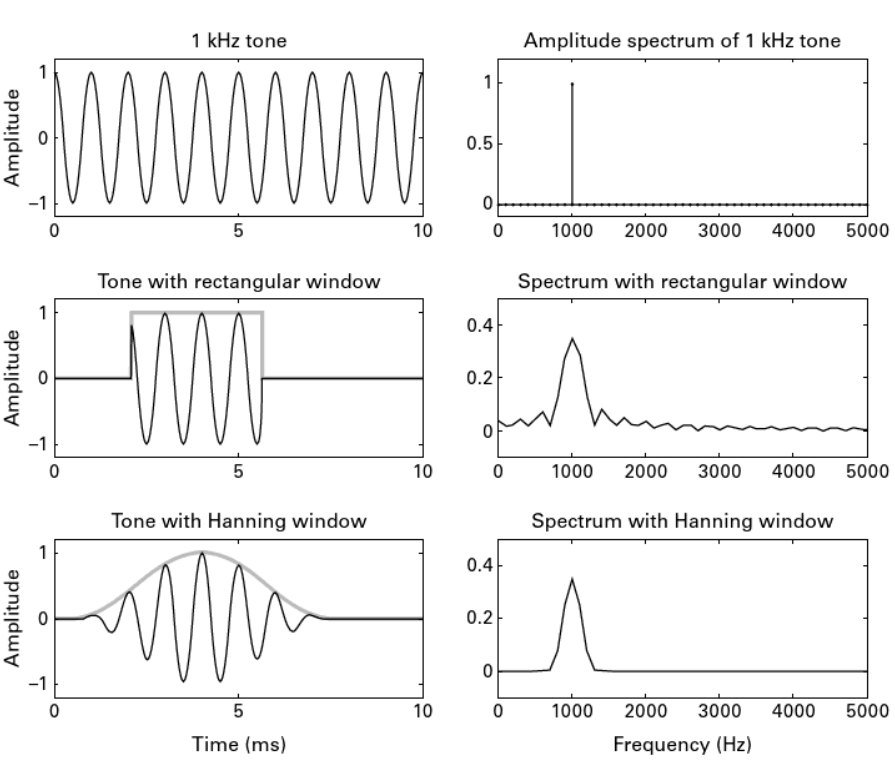
\includegraphics[width=0.75\textwidth]{include/windowing_example}
	\caption[An example of windowing and the problem of discontinuities]{The problem of discontinuities that arises when rectangular windows are used. The first row depicts a 1\,kHz pure tone (a sine wave) and its amplitude spectrum. The second row demonstrates the amplitude spectrum of the same tone masked by a rectangular window. The third row shows the spectrum of the same tone masked by a Hanning window. The window functions are shown in gray. Taken from \cite{Schnupp2011}.}
	\label{img:windowing_example}
\end{figure}

It is also worth noting that when the masking window is short, the resulting amplitude spectrum becomes wider, and vice versa: when the precise frequency representation is needed, the time window must be wide enough. This property is called time-frequency trade-off and can be observed in spectrograms: the spectrograms with high frequency resolution usually have low time resolution, and the ones with high time resolution have low frequency resolution.

\section{Filters and Filterbanks}\label{section:math_filters}

In chapter \ref{section:physics_sound}, when there was a conversation about the objects' impulse responses, some attention was given to the selectivity of frequencies. It was said that frequencies that don't align with the object's resonance frequency are attenuated, or filtered out. Thus, the mentioned object might be thought of as a mechanical linear filter. The linearity comes from the fact that the force applied to the object is proportional to the amplitude of the output signal (in simple words, the harder you pluck the guitar string, the louder the resulting sound will be). The linear filter's impulse response is a function of time that depicts how it responds to a simple external impulse, and its frequency response is a function that shows how much different frequencies are affected after the filtering.\\

The filters used in the implementation part of the thesis are digital, meaning that they ope\-rate on discrete-time or digital signals by performing different mathematical operations. Their counterpart is analog filters operating on continuous-time (also called analog) signals \cite{Shenoi2005}. Linear filters might be of two types: infinite impulse response (IIR) or finite impulse response (FIR). Impulse response of an IIR filter does not become equal to zero after a certain point in time, but continues infinitely, whereas impulse response of an FIR filter is given only for a certain time interval. FIR filters are usually non-recursive and less efficient, while IIR filters are recursive and computationally better.\\

The technique that is used for filtering of signals is called convolution. For digital signals, it is defined as follows \cite{Schnupp2011}:
\begin{equation}
	(f*g)(n) = \sum_{m=0}^{N-1}f(m)g(n - m) = \sum_{m=0}^{N-1}f(n - m)g(m)
\end{equation}
where $f(n)$ is the input signal, $g(n)$ is the filter impulse response, $m$ is the delay, or lag, and $N$ is the overall number of samples. Convolution is commutative, thus the functions for the input signal and the filter impulse response may be swapped.\\

The last term for this section is a filterbank. Basically, a filterbank is a collection of filters with different properties. In the implementation part, a filterbank of gammatone filters is used to simulate the basilar membrane of the human inner ear.

\section{Mathematical Concepts Used in the Thesis}\label{section:math_concepts}

This section will provide more specific information about the mathematical concepts used in the implementation part. They are listed below.

\begin{description}
	\item[Equivalent rectangular bandwidth] Equivalent rectangular bandwidth, or ERB, is a measure used for computing bandwidths of the filters for human auditory system. It was defined by Moore and Glasberg in 1983 as \cite{Moore1983}\cite{Holdsworth1988}:
	\begin{equation}
		ERB(f) = 6.23f^2 + 93.39f + 28.52
	\end{equation} 
	
	In 1990, the authors published another approximation (linear) \cite{Moore1990}\cite{Wang2006}:
	\begin{equation}
		ERB(f) = 24.7\,(4.37f + 1)
	\end{equation}
	
	\item[ERB-rate scale] In psychoacoustics, ERB-rate scale is used to uniformly distribute the filter center frequencies based on their ERB bandwidths. This scale is similar to the critical-band scale of the human auditory system. In 1983, Moore and Glasberg defined it as follows \cite{Moore1983}:
	\begin{equation}
		E(f) = 11.17\ln\left|\frac{f + 0.312}{f + 14.675}\right| + 43.0
	\end{equation}
	
	Using the latest approximation of ERB by Moore and Glasberg (1990), ERB-rate scale function is approximated as \cite{Moore1990}\cite{Wang2006}:
	\begin{equation}
		E(f) = 21.4\log_{10}\left(0.00437f + 1\right)
	\end{equation}
	
	\item[Gammatone filter] Gammatone filter is a linear filter, whose impulse response is a product of a sinusoidal tone and gamma function \cite{Wang2006}:
	\begin{equation}
		g_{f_c}(n) = at^{L-1}\,e^{-2\pi{}nb(f_c)}\,\cos(2\pi{}f_c{}n + \varphi)\,u(n)
	\end{equation}
	where $a$ is the filter amplitude, $L$ is its order (number of iterations of filtering), $f_c$ is its center frequency, $\varphi$ is the phase, $u(t)$ is the unit step function ($u(t) = 1$ for $t \ge 0$, and $0$ otherwise), and $b(f_c)$ is the function that determines the bandwidth for a given center frequency \cite{Wang2006}:
	\begin{equation}
		b(f) = 1.019\,ERB(f)
	\end{equation}
	
	Gammatone frequency response is defined as follows \cite{Holdsworth1988}:
	\begin{equation}
		G(f) = \left[1 + \frac{j\,(f - f_c)}{b(f_c)}\right]^{-L} + 
		\left[1 + \frac{j\,(f + f_c)}{b(f_c)}\right]^{-L}
		\qquad\left(-\infty < f < \infty\right)
	\end{equation}
	
	However, when modeling human auditory system, the second term from the definition above can be ignored for sufficiently large $\frac{f_c}{b(f_c)}$ \cite{Wang2006}\cite{Holdsworth1988}:
	\begin{equation}
		G(f)\approx\left[1 + \frac{j\,(f - f_c)}{b(f_c)}\right]^{-L}
		\qquad\left(0 < f < \infty\right)
	\end{equation}
	
	\item[Autocorrelation] Autocorrelation, or autocorrelation function (ACF), is a function that is used to find periodicities and other cues in the input signal. It is defined as the correlation of the signal with its shifted copy, and in this thesis the simulated auditory nerve responses will be used \cite{Wang2006}:
	\begin{equation}
		ACF(n, c, \tau) = \frac{
			\sum\limits_{k=0}^{K-1}a(n - k, c)\,a(n - k -\tau, c)
		}{
			\sqrt{\strut\sum\limits_{\tau}{a(n - k, c)^2}}\,
			\sqrt{\strut\sum\limits_{\tau}{a(n - k - \tau, c)^2}}
		}\,h(k)
	\end{equation}
	where $a(n, c)$ represents the simulated auditory nerve response for frequency channel $c$ and discrete time $n$, $\tau$ is the time lag, $K$ is the length of the sampling window, and $h(k)$ is the window function (usually Hanning, exponential or rectangular).
	
	\item[Summary autocorrelation] Summary autocorrelation function, or SACF, is defined as \cite{Wang2006}\cite{Virtanen2012}:
	\begin{equation}
		SACF(n, \tau) = \sum_c{ACF(n, c, \tau)}
	\end{equation}
	
	\item[Cross-channel correlation] Cross-channel correlation is a correlation between signals from different frequency channels. In this thesis it is defined only for each two neighboring channels ($c$ and $c + 1$) using autocorrelation function \cite{Virtanen2012}: 
	\begin{equation}
		CCF(n, c) = \frac{
			\sum\limits_{\tau}{
				\left[ACF(n, c, \tau) - \overline{ACF(n, c)}\right]
				\left[ACF(n, c + 1, \tau) - \overline{ACF(n, c + 1)}\right]}
		}{
			\sqrt{\strut\sum\limits_{\tau}{
				\left[ACF(n, c, \tau) - \overline{ACF(n, c)}\right]^2}}\,
			\sqrt{\strut\sum\limits_{\tau}{
				\left[ACF(n, c + 1, \tau) - \overline{ACF(n, c + 1)}\right]^2}}
		}
	\end{equation}
	where $\overline{ACF(n, c)}$ is the mean $ACF$ over $\tau$.
\end{description}
